\chapter*{Clustering}
\setcounter{chapter}{1}
We clustered our data containing letters with a set of their attributes using
Gaussian Mixture Model as well as with Hierarchical clustering. We used
cross-validation to estimate the optimal parameters for both algorithms. At
the end we estimated the quality of both algorithms in terms of our true labels
which are letters.


\section{Gaussian Mixture Model (GMM)}
For GMM algorithm we used double cross-validation to estimate the best number of
components in internal loop and calculating quality score in external loop as
an average of scores. We also applied Principal Component Analysis to visualize
the results in more human friendly way. We used only a subset of our dataset for
performance reasons, using random sampling. We can see the results in the figure
\ref{fig:GMM}
\begin{figure}[!tbh]
  \centering
  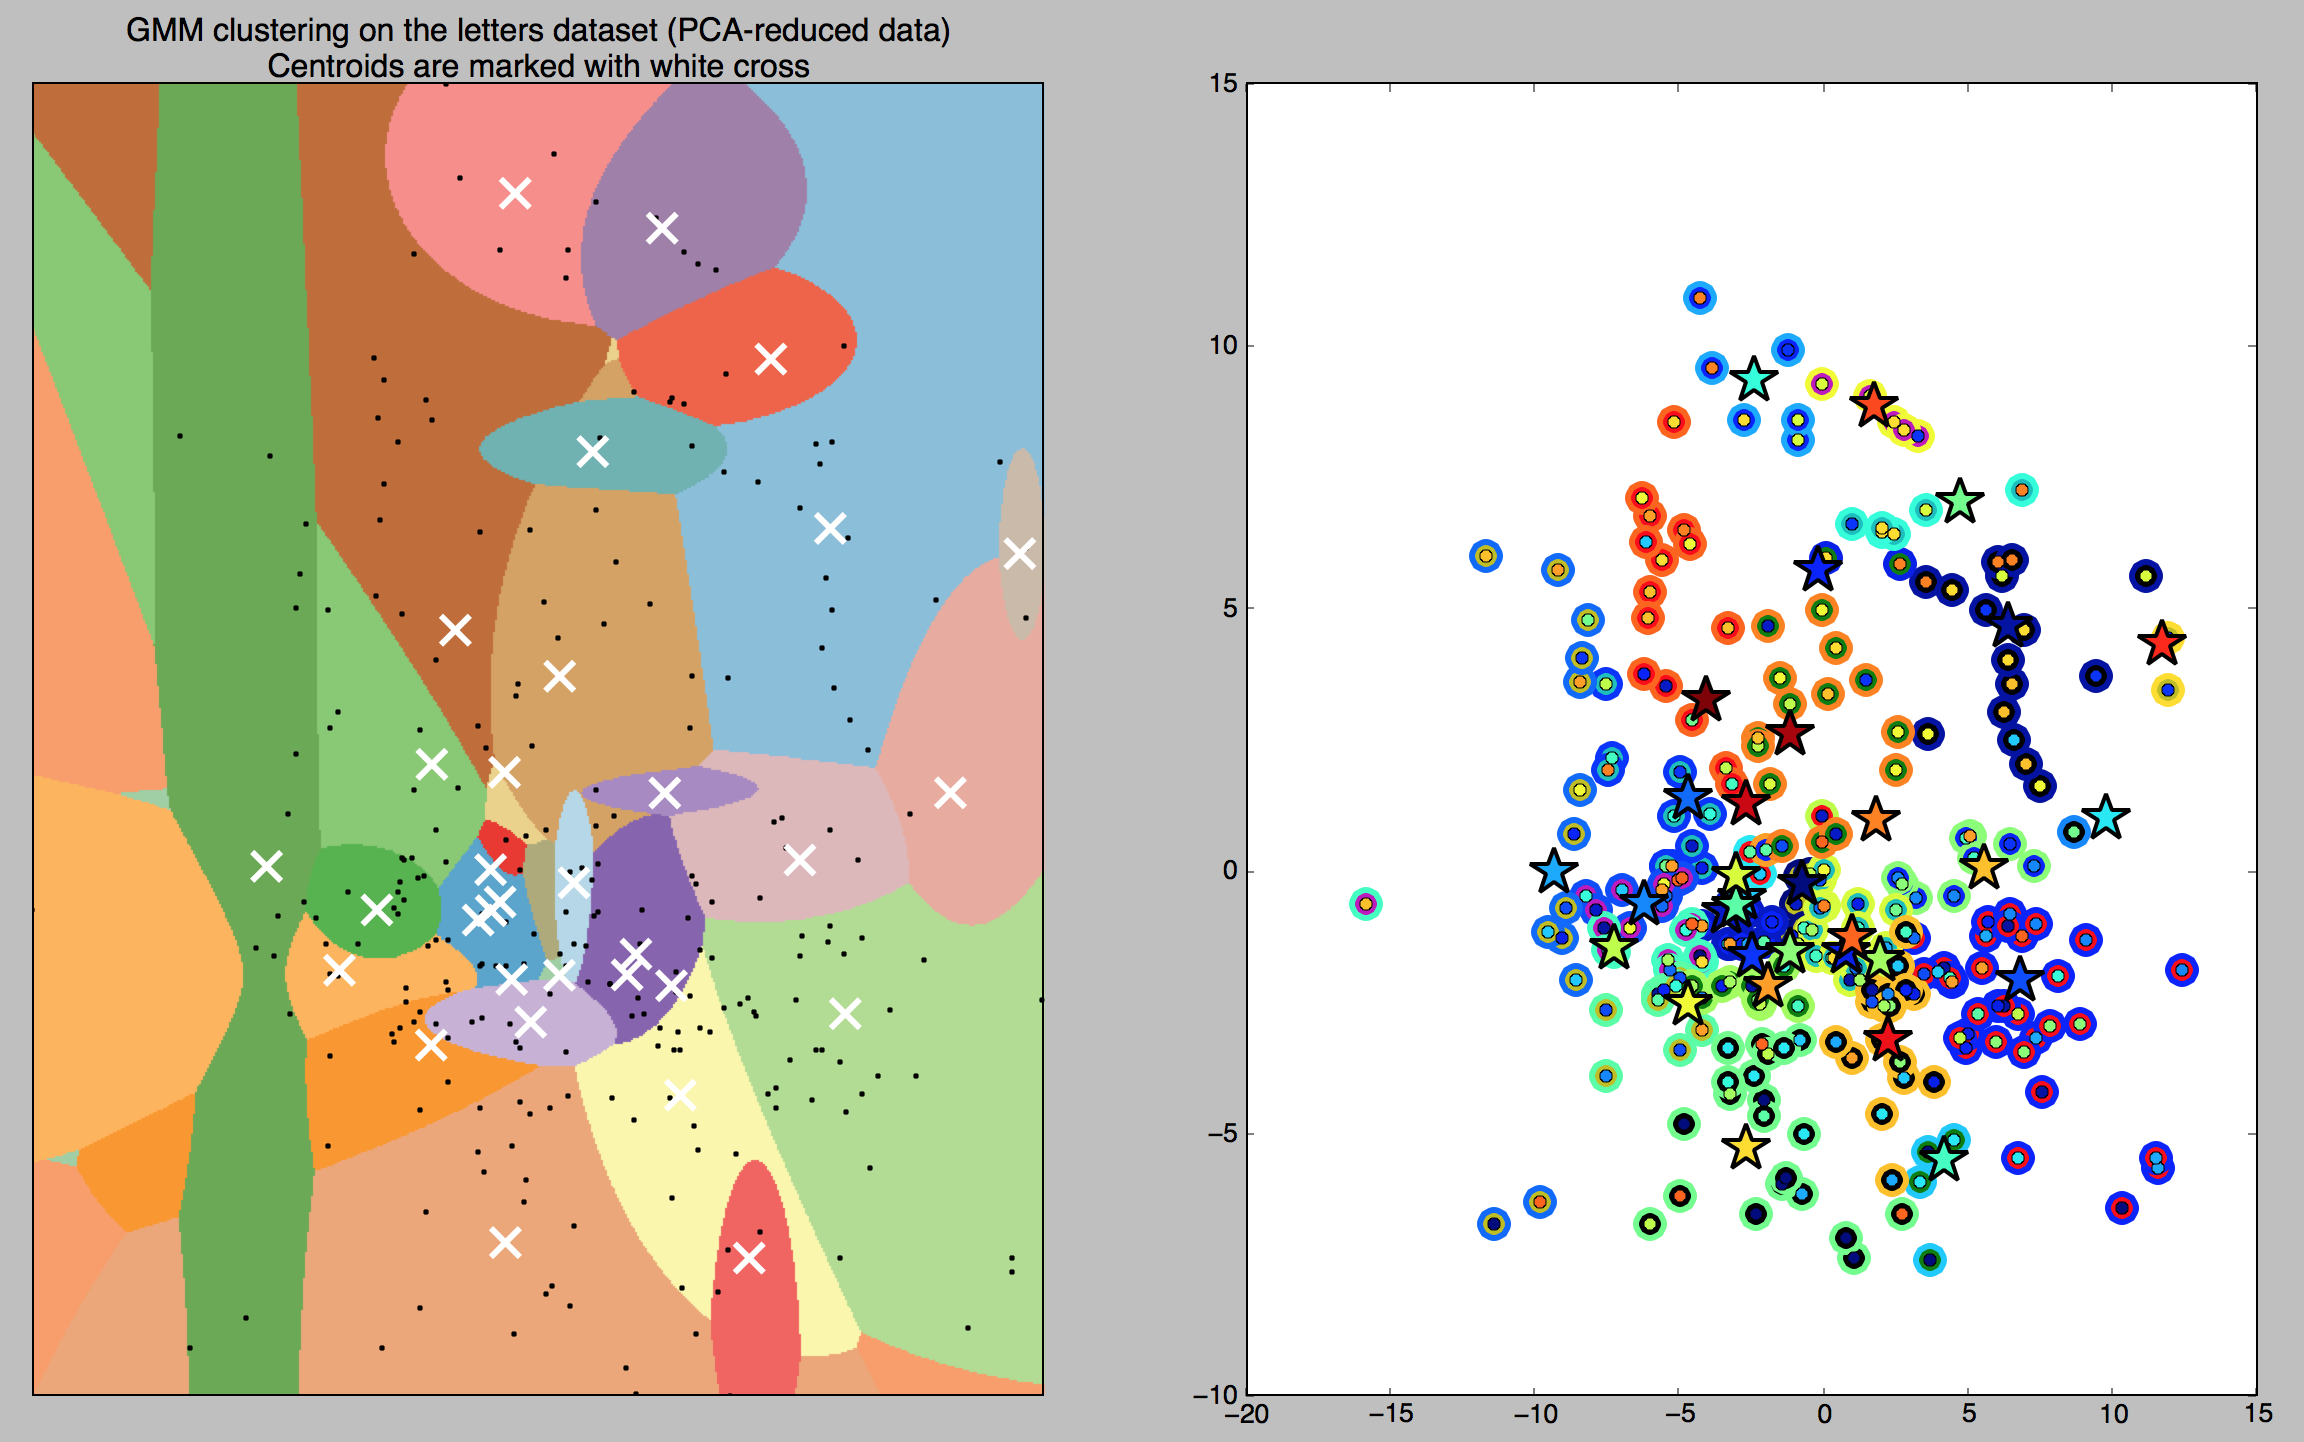
\includegraphics[width=0.6\textwidth]{figures/GMM_pca_2_2}
  \caption{GMM - clustered (data reduced using PCA)}
  \label{fig:GMM}
\end{figure}
In an average the most optimal number of components choosed in internal
cross-validation loop was 30. Which is a close to the number of actual classes.
We can see how the quality of GMM clustering in terms of actual labels depends
on the number of components in the figure \ref{fig:ami}
\begin{figure}[!tbh]
  \centering
  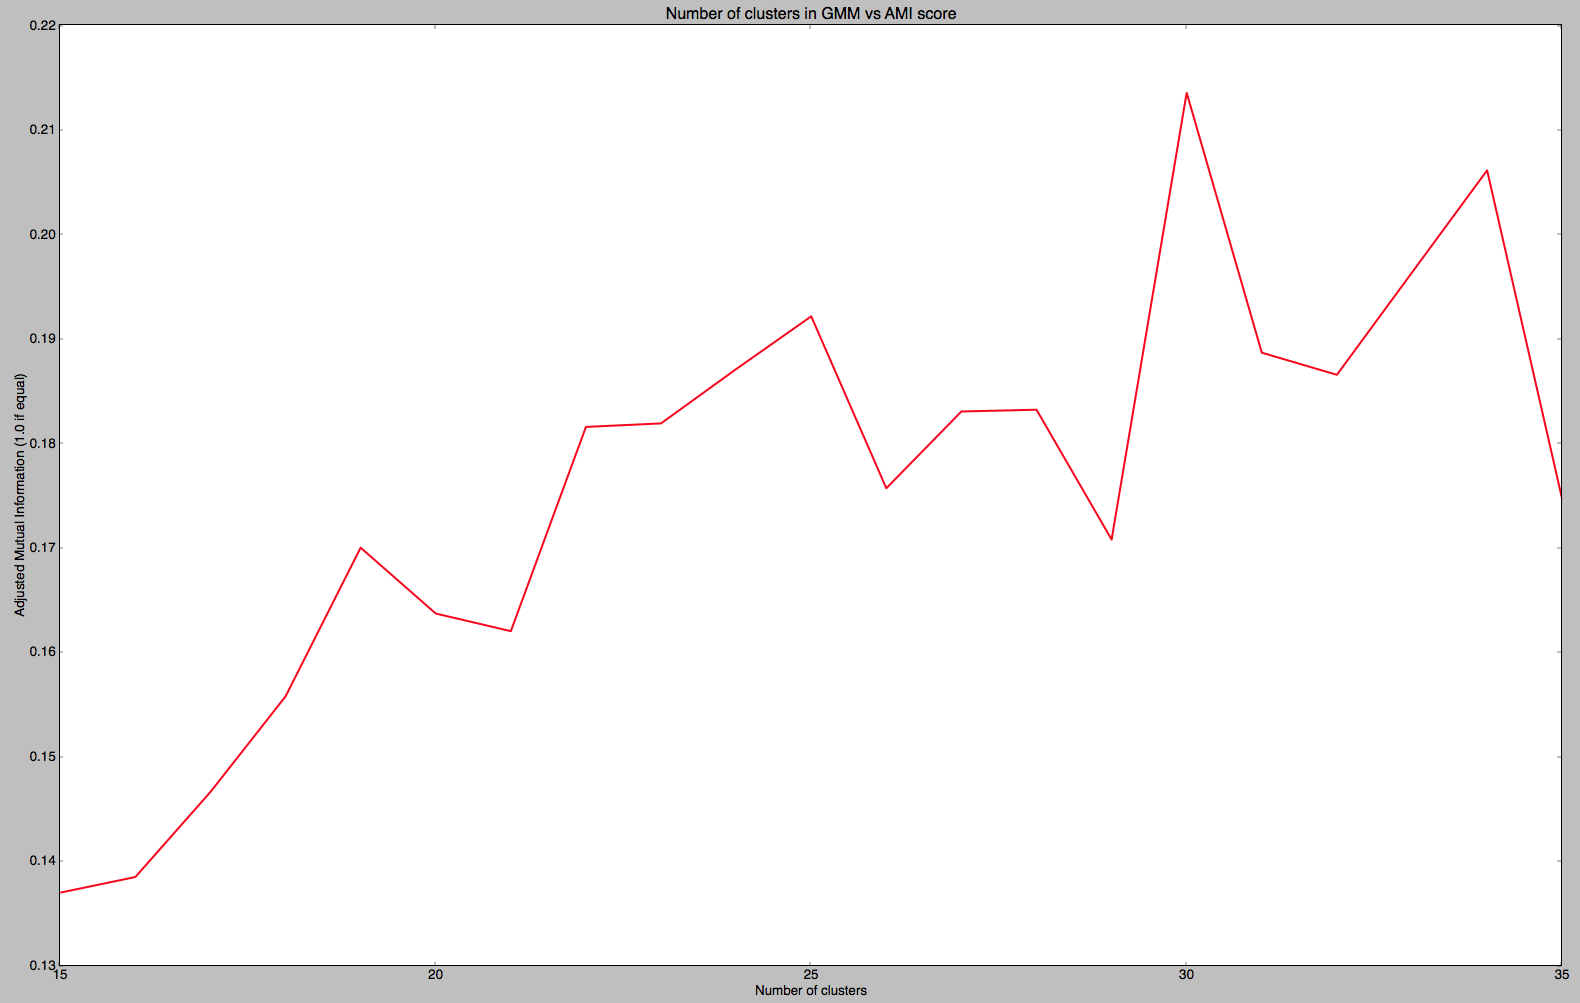
\includegraphics[width=0.6\textwidth]{figures/ami}
  \caption{GMM - quality vs components count}
  \label{fig:ami}
\end{figure}
Cluster centers should be in ideal case (especially if we consider number of
components equal to the number of actual classes - 26) an average vector from
the attribute vectors corresponding to particular letters. So the centroids
should correspond to some ,,unified'' letters.

\section{Hierarchical Clustering}
We also used single cross-validation technique in Hierarchical Clustering and
choose the best metric and linkage function from all available options. Score
results are mesured for best performing option sets. We also used PCA to help
visualize results (Figure~\ref{fig:hier_all} and Figure~\ref{fig:hier_pca}).
\begin{figure}[!tbh]
  \centering
  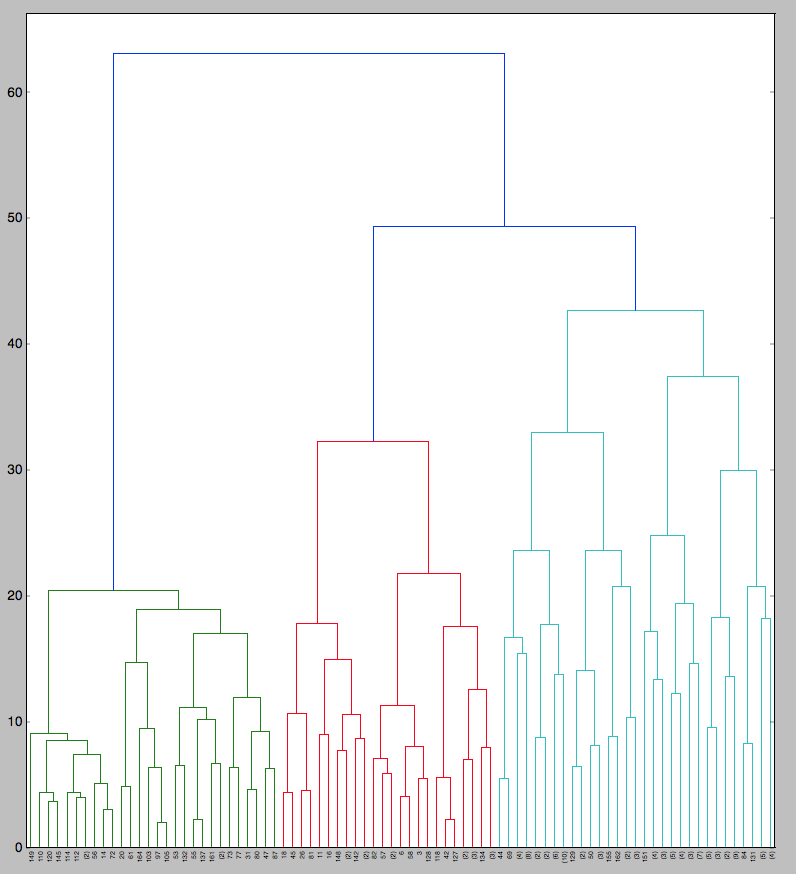
\includegraphics[width=0.6\textwidth]{figures/Hier_all_1}
  \caption{Hierarchical clustering (without PCA reduction)}
  \label{fig:hier_all}
\end{figure}
\begin{figure}[!tbh]
  \centering
  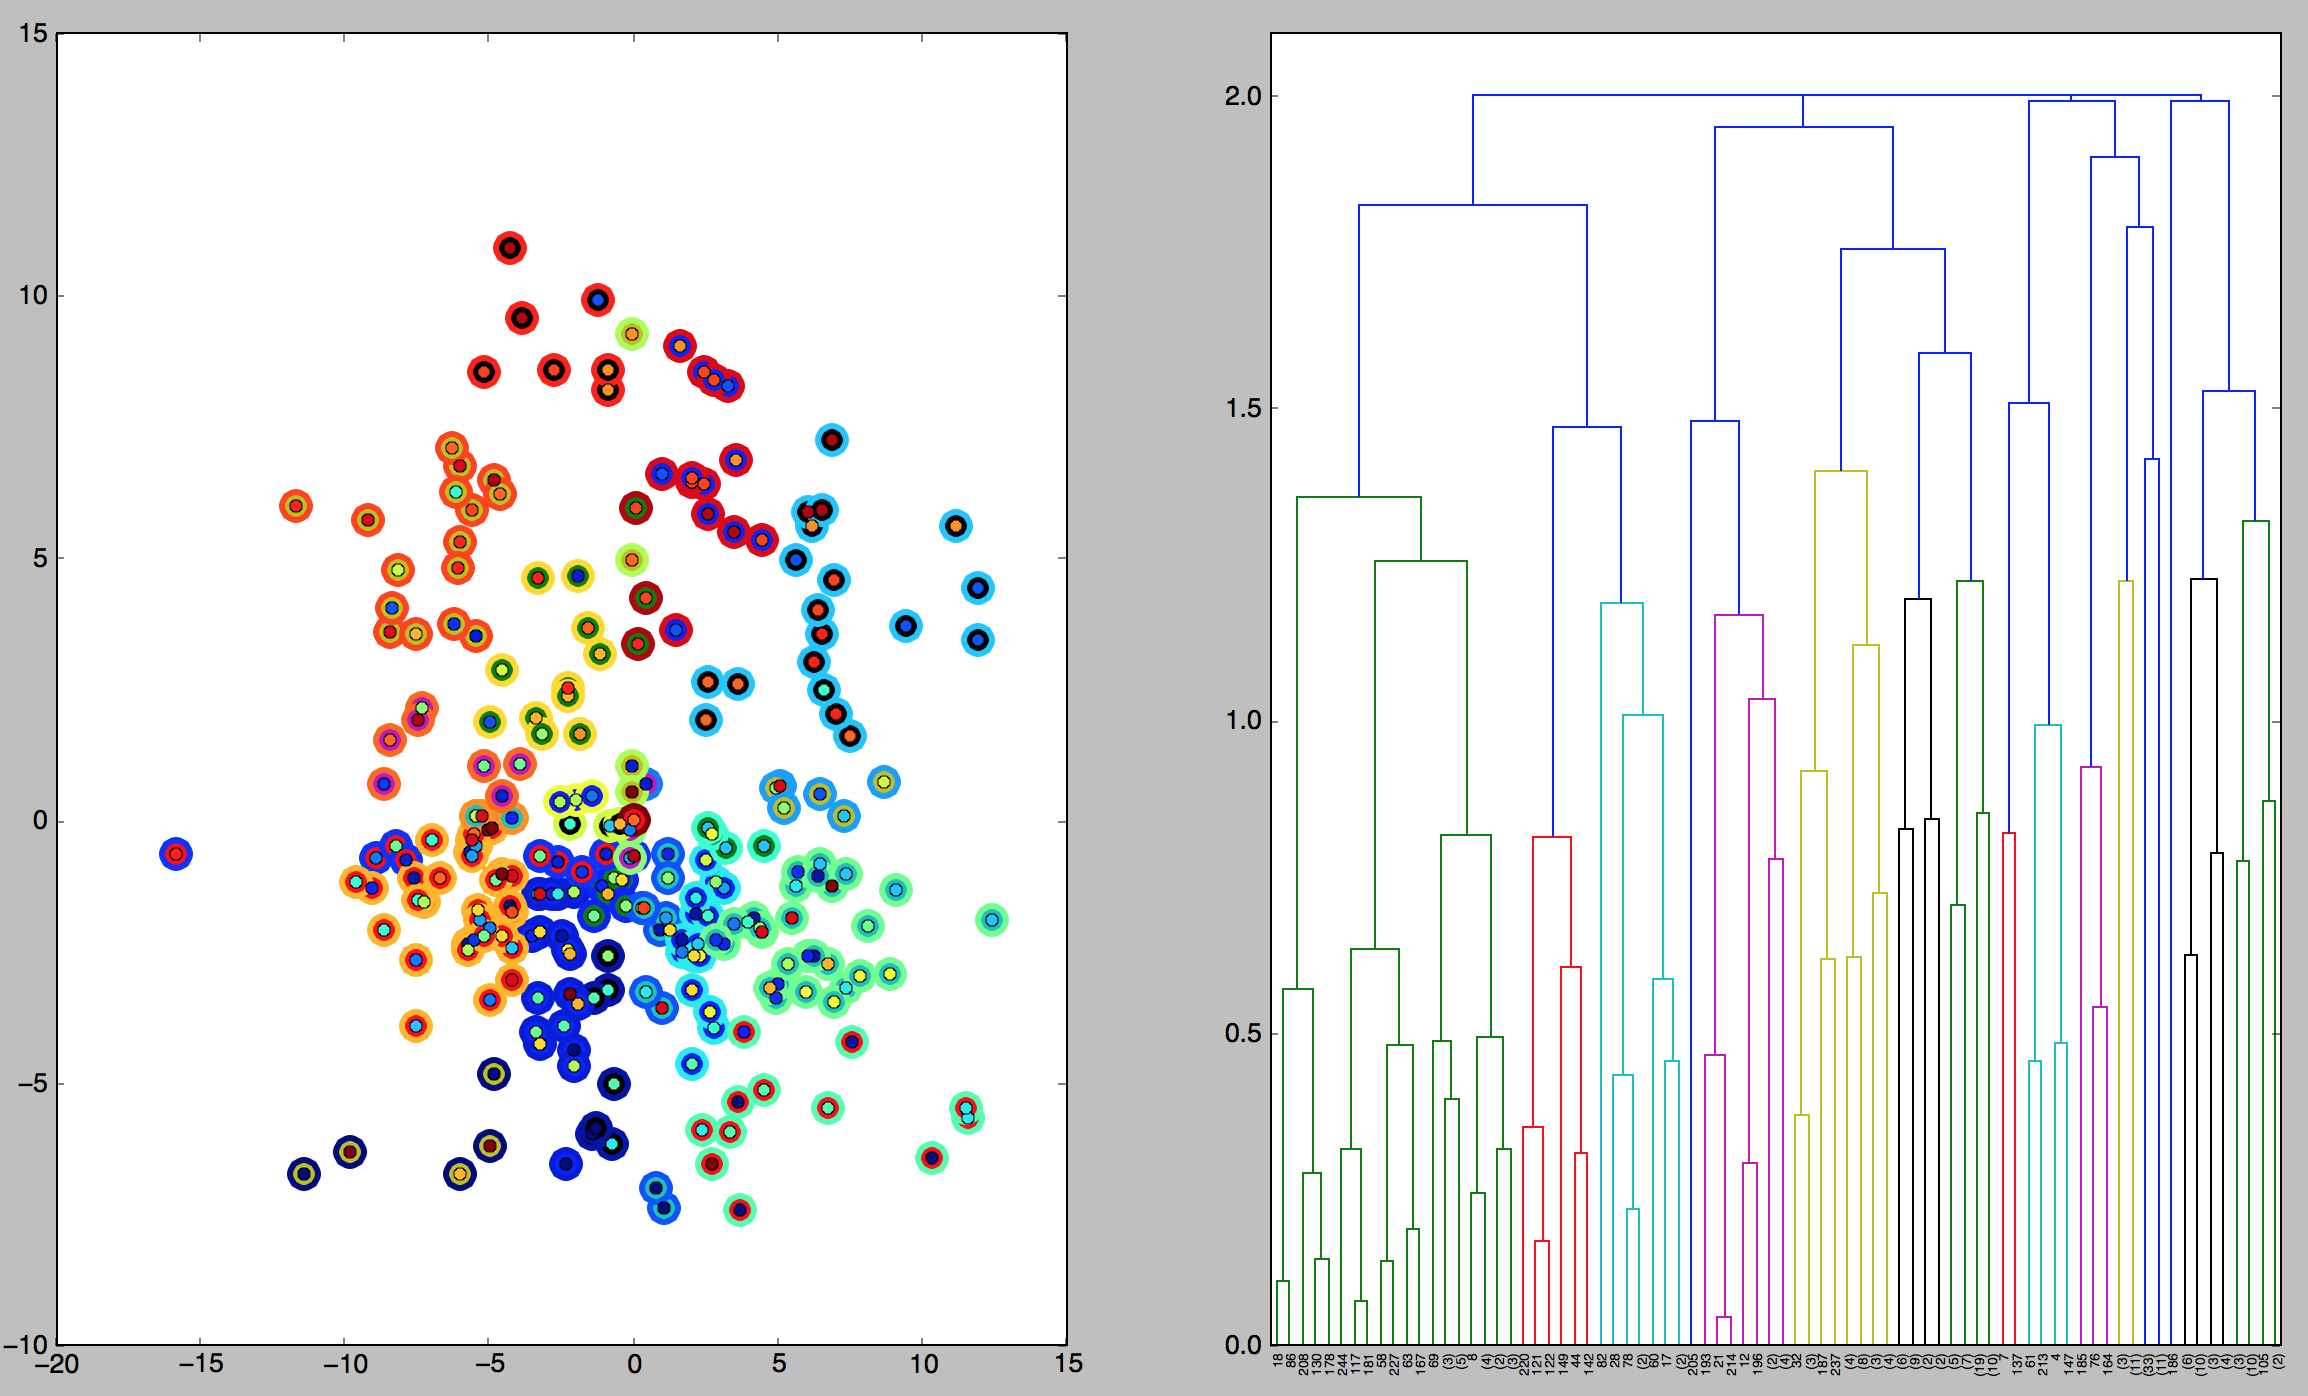
\includegraphics[width=0.6\textwidth]{figures/Hier_pca_2_1}
  \caption{Hierarchical clustering (data reduced using PCA)}
  \label{fig:hier_pca}
\end{figure}
Even using first two principal components explaining the most variance, results
are dyrastically worse than when we use all data dimensions. The most commonly
choosed options by the program were ('ward', 'euclidean') which means that the
ward linkage function and euclidean metric were most suitable for our data.

\section{Evaluation}
We choosed an adjusted mutual info score metric as our quality messure for
clustering methods. For two clusterings U and V, the AMI is given as:
$$ AMI(U, V) = [MI(U, V) - E(MI(U, V))] / [max(H(U), H(V)) - E(MI(U, V))] $$
And has following properties:
\begin{enumerate}
\item Perfect labeling is scored 1.0
\item Independent labelings have non-positive scores
\item No assumption is made on the cluster structure
\item It is symmetric
\item It is independent of the absolute values of the labels: a permutation of
      the class or cluster label values won’t change the score value in any way
\item It accounts for the fact that the MI is generally higher for two
      clusterings with a larger number of clusters, regardless of whether there
      is actually more information shared
\end{enumerate}

Reaserch has shown that Hierarchical clustering performs better for our data
than GMM and also that both methods have better scores while having more data.
However it was impossible for performance reasons to run this methods on more
than 3000 records of our data, where results would be even better. It is
visualized in the figure \ref{fig:scores}
\begin{figure}[!tbh]
  \centering
  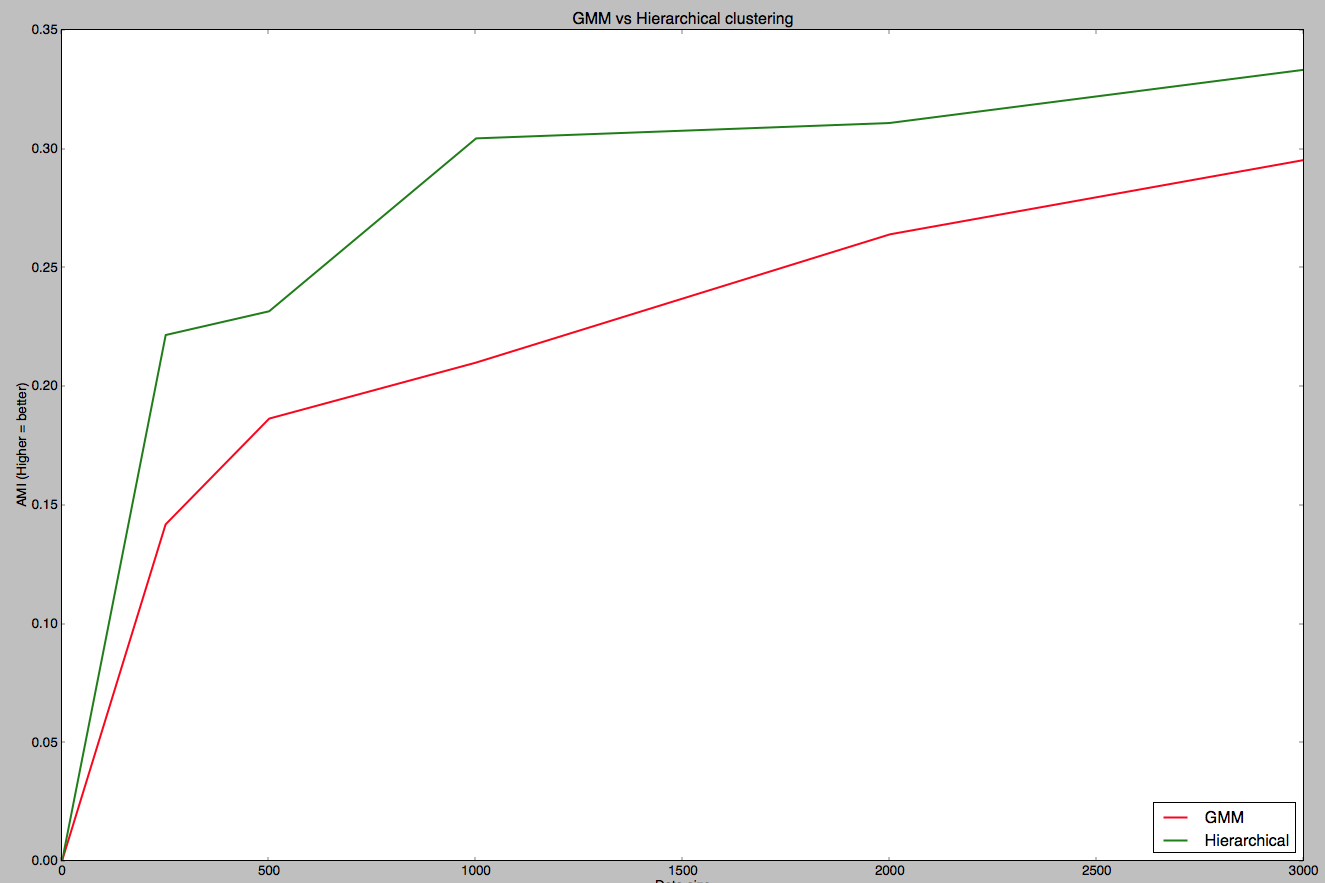
\includegraphics[width=1.0\textwidth]{figures/scores}
  \caption{GMM vs Hierarchical clustering quality}
  \label{fig:scores}
\end{figure}
